\documentclass[a4paper]{article}

\usepackage[pdftex]{graphicx}
\usepackage[margin=3cm]{geometry}
\usepackage{verbatim,moreverb,amssymb,amsmath,paralist}
\usepackage[noend]{algorithmic}

\algsetup{indent=2em}
\renewcommand{\algorithmiccomment}[1]{\quad \{\emph{#1}\}}


\newcounter{question}
\newcommand{\question}[1]{\refstepcounter{question}\section*{Question~\thequestion~~~\small\emph{(#1)}}}
\renewcommand*\thequestion{\arabic{question}}


\begin{document}

\pagestyle{empty}
\thispagestyle{empty}



\noindent
\begin{minipage}{\columnwidth}
  \centering
  \Large
  DA4002 (HT13) Halmstad University\\
  Introduction to Algorithms, Data Structures, and Problem Solving\\[3\baselineskip]
  \Huge
  Written Exam\\
  \Large
  Friday, November 1, 2013\\[2\baselineskip]
  Examiner: Roland Philippsen
\end{minipage}

\vfill

\noindent
\begin{center}
\fbox{
  \begin{minipage}{0.8\columnwidth}
    \textbf{Student Name:}\\[3\baselineskip]
  \end{minipage}
}
\end{center}

\vfill



\section*{Rules}

Aside from the obvious rules of conduct exams (e.g.\ no chatting):

\begin{itemize}
\item
  \textbf{No computing devices} (laptops, phones, calculators, \emph{etc}).
\item
  \textbf{No books or printouts} except for non-electronic dictionaries.
\item
  \textbf{Allowed hand-written notes}: two sheets of A4 paper (front and back).
\end{itemize}



\section*{General Guidelines}

\begin{itemize}
\item
  \textbf{Read carefully} and pace yourself.
  You can solve the problems in any order you want, but later problems may be easier to solve after you have answered the preceding questions.
\item
  \textbf{Write clearly} and draw clear diagrams.
  If you need to correct a mistake, then cleanly cross out the wrong answer and clearly indicate where the correction can be found.
\item
  \textbf{Indicate the question number} for each of your answers.
  If a question has sub-questions, indicate the sub-question number after the main question number, separated by a dot.
  For example, question 3 has 4 sub-questions, and their answers should be numbered 3.1, 3.2, 3.3, and 3.4.
\end{itemize}



\pagebreak
\pagestyle{plain}
\thispagestyle{plain}
\setcounter{page}{1}



\question{6 points}

In the following table, match the data structure names with the diagrams \textbf{(A, B, or C)}, and the code segments \textbf{(X, Y, or Z)}.

\vfill

\begin{center}
  \begin{tabular}{|l|*2{p{0.25\columnwidth}|}}
    \hline
    \emph{data structure} & \emph{diagram (A, B, or C)} & \emph{code (X, Y, or Z)} \\
    \hline
    simply linked list & & \\
    \hline
    doubly linked list & & \\
    \hline
    simply linked circular list & & \\
    \hline
    doubly linked circular list & & \\
    \hline
    binary tree & & \\
    \hline
    sibling-child tree & & \\
    \hline
  \end{tabular}
\end{center}

\vfill

\begin{center}
  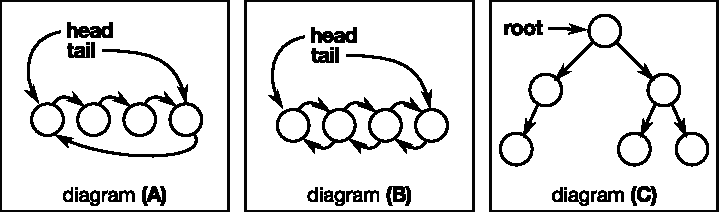
\includegraphics[width=0.8\columnwidth]{q1diag.pdf}
\end{center}

\vfill

\noindent
\begin{minipage}{0.42\columnwidth}
  \fbox{\begin{minipage}{\columnwidth}
      code segment \textbf{X}:
      \small
      \verbatiminput{q1x.c}
  \end{minipage}}
  \fbox{\begin{minipage}{\columnwidth}
      code segment \textbf{Z}:
      \small
      \verbatiminput{q1z.c}
  \end{minipage}}
\end{minipage}
\hfill
\fbox{\begin{minipage}{0.52\columnwidth}
    code segment \textbf{Y}:
    \small
    \verbatiminput{q1y.c}
\end{minipage}}

\clearpage

\question{4 points}

\begin{enumerate}
\item
  What is the the Big-Oh $O(N)$ expressions for the following runtime formula $T_1(N)$?
  \begin{equation*}
    T_1(N) = N \left( 12\log N + \sum_{i=1}^Ni \right) + 0.1 N^2
  \end{equation*}
\item
  What is the the Big-Oh $O(N)$ expressions for the following runtime formula $T_2(N)$?
  \begin{equation*}
    T_2(N) =
    \begin{cases}
      1          & \text{for} N \leq 1 \\
      2 T_2(N/2) & \text{otherwise}
    \end{cases}
  \end{equation*}
\item
  What is the Big-Oh $O(N)$ expression for the runtime $T_3(N)$ of the following code segment?\\[1.5\baselineskip]
  \fbox{\begin{minipage}{0.8\columnwidth}
      \small
      \verbatiminput{q2a.c}
  \end{minipage}}\\[2\baselineskip]
\item
  What is the Big-Oh $O(N)$ expression for the runtime $T_4(N)$ of the following code segment?\\[1.5\baselineskip]
  \fbox{\begin{minipage}{0.8\columnwidth}
      \small
      \verbatiminput{q2b.c}
  \end{minipage}}
\end{enumerate}



\clearpage

\question{6 points}

Do a bunch of runtime estimates given big-Oh expressions.

\vfill

\noindent
\begin{tabular}{|l|r|r|r|r|r|r|r|r|r|r|r|r|r|r|r|}
  \hline
  $x=$   & 0 & 1 & 2 &  3 &  4 &   5 &   6 &   7 &   8 &   9 &   10 &   11 &   12 &   13 &    14 \\
  $x^2=$ & 0 & 1 & 4 &  9 & 16 &  25 &  36 &  49 &  64 &  81 &  100 &  121 &  144 &  169 &   196 \\
  $x^3=$ & 0 & 1 & 8 & 27 & 64 & 125 & 216 & 343 & 512 & 729 & 1000 & 1331 & 1728 & 2197 &  2744 \\
  $2^x=$ & 1 & 2 & 4 &  8 & 16 &  32 &  64 & 128 & 256 & 512 & 1024 & 2048 & 4096 & 8192 & 16384 \\
  \hline
\end{tabular}



\clearpage

\question{5 points}

A positive-weighted directed graph is a graph where edges have a direction as well as an associated cost.
A minimum-cost path in such a graph is a path from a \emph{start} node to a \emph{goal} node such that the sum of edge costs along this path is minimum.

\begin{enumerate}
\item
  Draw a diagram representing the graph given in the adjacency matrix below.
  The existence of edges as well as their cost are directly given by the non-empty entries in the matrix.
  In your diagram, also indicate the cost of each edge on the diagram.
  Note that for the next question, you will also need to indicate a value for each node, so leave enough room for this.
\item
  Run the graph algorithm explained below on the given graph, starting at node \textbf{B}.
  This is ``Dijkstra's Algorithm'' which computes the value of minimum-cost paths from a given start node to all other nodes in the graph.
  Write the resulting node values into the your graph diagram.
\item
  What is the minimum-cost path from \textbf{B} to \textbf{D}?
  What is its cost, and what is the sequence of visited nodes?
\end{enumerate}

\vfill

\begin{center}
  \begin{minipage}{0.45\columnwidth}
    \begin{tabular}{|*{6}{c|}}
      \hline
      \emph{source}
      &
      \multicolumn{5}{l|}{\emph{destination}} \\
        &  A &  B &  C &  D &  E \\
      \hline
      A &    &  2 &    &  1 &    \\
      \hline
      B &    &    &  5 &    &  4 \\
      \hline
      C &    & 10 &    &  6 &    \\
      \hline
      D &    &    &  2 &    &  2 \\
      \hline
      E &  4 &    &    &  7 &    \\
      \hline
    \end{tabular}
  \end{minipage}
  \fbox{\begin{minipage}{0.45\columnwidth}
      \begin{algorithmic}[1]
        \FORALL { nodes $n$ }
          \STATE $v(n) \leftarrow \infty$
        \ENDFOR
        \STATE $v(s) \leftarrow 0$
        \STATE $\text{insert}(Q,s)$
        \WHILE { $0 \neq \text{length}(Q)$ }
          \STATE $n \leftarrow \text{extract}(Q)$
          \FORALL { $e=(n,m)$ }
            \IF { $v(m) > v(n) + c(e)$ }
              \STATE $v(m) \leftarrow v(n) + c(e)$
              \STATE $\text{insert}(Q,m)$
            \ENDIF
          \ENDFOR
        \ENDWHILE
      \end{algorithmic}
  \end{minipage}}
\end{center}

\vfill

\noindent\textbf{Detailed explanations about the pseudo-code:}

Left-pointing arrows denote assignment.
For example ``$x \leftarrow 1$'' means that the value 1 is stored into the variable $x$.
Nodes are written $n$ or $m$.
The start node is written $s$.
Each node has a value, which is written $v(n)$.
Edges are written $e=(n,m)$ which means that there is an edge from node $n$ to node $m$.
Edge costs are written $c(e)$.

$Q$ denotes a priority queue that contains nodes $n$ sorted by their value $v(n)$.
It supports the following operations:
\begin{compactitem}
\item
  $n \leftarrow \text{extract}(Q)$ removes the node with the smallest value from the queue.
\item
  $\text{insert}(Q,n)$ inserts the node $n$ into the queue.
  If $n$ is already in the queue, then its place in the queue gets updated.
\item
  $\text{length}(Q)$ is the number of nodes in the queue.
\end{compactitem}

Lines 1--4 perform initializations: all values are set to infinity, except the start node which gets a value of zero.
Also, the queue is initialized to contain just the start node.

The outer loop (lines 5--10) runs until the queue is empty.
Line 6 retrieves the queued node with the smallest value.
This node $n$ is the \emph{source} used by the inner loop.

The inner loop (lines 7--10) runs over all \emph{destination} nodes that can be reached from the source.
Line 8 checks whether a destination can be more cheaply reached from the current source.
If that is the case, then lines 9--10 update the destination by lowering its value, and inserting it into the queue.



\clearpage

\question{6 points}

Imagine that your are working as a programmer and encounter the following situations.

\begin{enumerate}
\item
  One of your colleagues wants to speed up an existing program that manages information about persons.
  The program currently keeps the information in a linked list.
  This list is only rarely modified, but very frequently used to search for persons.
  Your colleague plans to change the program so that it sorts the list, and then uses binary search instead of linear search.
  Do you think this is a good idea?
  Why, or why not?
\item
  Another colleague, working on a similar but different program, has written functions for saving the data from a binary search tree in a file and later loading them back from the file.
  He implemented the safe function using in-order traversal, and everything worked correctly and quickly during his tests with small data sets.
  However, with large data sets, the program becomes very slow after loading data from such a file.
  What do you think is going wrong?
  What do you suggest to solve this problem?
\item
  You are leading a team that works on designing and implementing an email routing system that is expected to handle a very large amount of messages.
  The idea is to use up to 10 priority levels so that important email gets sent first while less important messages wait.
  Your team has come up with three suggestions for implementing the message queue:
  \begin{compactitem}
  \item
    use a min heap with array-backed storage, sorted by priority level;
  \item
    use an array of 10 linked lists, one for each priority level;
  \item
    use a dynamically sized array.
  \end{compactitem}
  Which of these solutions would you choose, and why?
\end{enumerate}



\end{document}
